
\chapter{Properties of Motors and Muscles}
\label{sec:PropertiesOfMotorsAndMuscles}

Unfortunately, current technologies do not allow us to replicate the properties of muscles exactly. Muscles are strong and light, and can fit into extremely small spaces while still being able to deliver tremendous force. Muscles are a type of actuator, which may be defined as a system that converts energy from any form into motion (kinetic energy).The two most robust forms of man-made actuators in use today on legged robots are hydraulics and electric motors. Hydraulics are powerful, but they are extremely inefficient and can leak oil. Electric motors are far more efficient with energy, and thus are the main focus of actuation options in this text. This chapter starts with an introduction to the properties of electric motors and a discussion of their power consumption. The section on electric motors is followed by an introduction to human locomotive muscle properties, and how these muscles compare to electric motors.

\section{Motors} % (notes page 3-7)
\label{IntroductionToMotors}
\index{motors}

Generally speaking, using stored electricity to power electric actuators is extremely efficient. One \unit{Joule} of stored electric energy, in either a battery or capacitor, will deliver almost one \unit{Joule} of energy to an electric motor paired with the storage device. This is greatly different from combustion-driven actuators, for which the amount of energy stored in chemical bonds is approximately four times the amount of thermal energy that results from the combustion.
\par % trying Ruina's paragraph command
A basic configuration of an electric motor and a power supply is shown in figure \ref{fig:PowerSupplyAndMotor}. The voltage and current associated with the power supply are $V$ and $I$, respectively. The angular speed and torque provided by the motor are $\omega$ and $T$, respectively.

% FIGURE
\begin{figure}[h]		% h="here" t="top" b="bottom" p="separate page"
\begin{centering}
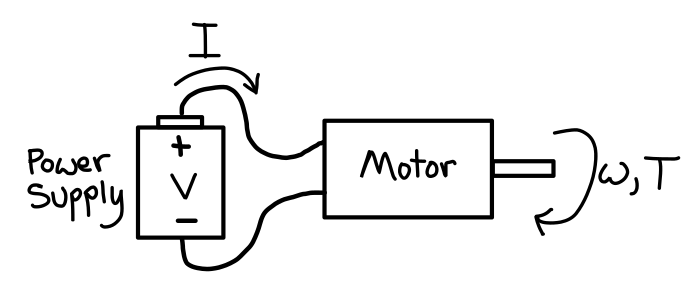
\includegraphics[width=0.5\textwidth]{Figures/PowerSupplyAndMotor}\par
\end{centering}
\caption[Diagram: Power Supply and Electric Motor]{Power supply and electric motor. The power supply provides $I$ Amperes of current at a potential difference of $V$ Volts. This creates $T$ Newton-meters of torque and spins the motor at $\omega$ radians per second.}
\label{fig:PowerSupplyAndMotor}
\end{figure}
%

We are interested in the relationships between $I$, $V$, $\omega$, and $T$. Given that we have four variables, we can choose one of them to control so that we are left with three equations that govern the other variables.

\subsection*{Power}
\label{sec:Power}

The power consumed and developed by the configuration shown in figure \ref{fig:PowerSupplyAndMotor} is described by the following equations:

\begin{equation}
P_{i}=P_{in} = \mbox{electric power into motor}= IV
\label{eq:PowerIn}
\end{equation}

\begin{equation}
P_{o}=P_{out} = \mbox{power motor exerts on environment} = T\omega
\label{eq:PowerOut}
\end{equation}

The fundamental restriction on electric motors is that there is always positive energy dissipation in the motor due to heat loss, and so power input from the battery is greater than power output by the motor. This holds true for many types of actuation systems, as it is nearly impossible to build a completely lossless, or ideal, machine or system. Figure \ref{fig:IdealPowerPlotSketch} demonstrates this fundamental restriction.

% FIGURE
\begin{figure}[h]		% h="here" t="top" b="bottom" p="separate page"
\begin{centering}
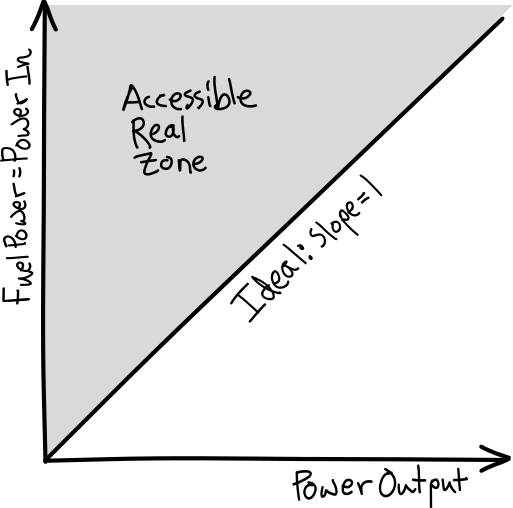
\includegraphics[width=0.5\textwidth]{Figures/IdealPowerPlotSketch}\par
\end{centering}
\caption[Plot: Power Conservation]{Fuel power input to a system vs. the power output by the system. An ideal system would produce as much power in the form of mechanical work as it consumes in chemical energy from fuel. The shaded area of this plot represents the performance levels attainable by real systems.}
\label{fig:IdealPowerPlotSketch}
\end{figure}
\index{power}

Imagine for one instant in time that $\omega$ is chosen or known. Perhaps this means that we want to set the speed at which a limb in a legged robot is rotating. This leaves the variables $T$, $V$, and $I$ to control in some way. If $V$ and $I$ are controlled, equations \ref{eq:PowerIn} and \ref{eq:PowerOut} can be combined in a power conservation equation:

\begin{equation}
IV = T\omega + I^{2} R
\label{eq:EnergyConservation}
\end{equation}

where the $I^{2}R$ term represents power dissipation from the internal resistance of the motor. Additionally, we can quantify the motor torque:

\begin{equation}
T = kI
\label{eq:MotorTorque}
\end{equation}

where $k$ is the motor torque constant, which has units of \unitfrac{Nm}{Amp}. Substitution of equation \ref{eq:MotorTorque} into equation \ref{eq:EnergyConservation}, gives the motor voltage law:

\begin{equation}
V = k\omega + IR
\label{eq:MotorVoltage}
\end{equation}

We think of equations \ref{eq:MotorTorque} and \ref{eq:MotorVoltage} as describing a motor that is controlled by a given voltage. So if given a voltage, say \unit[9]{Volts}, we would like to eliminate $I$ from these two equations so that we can see how the machine behaves. Manipulation yields:

\begin{equation}
V = k\omega + \frac{T}{k}R
\label{eq:MotorVoltage2}
\end{equation}

\begin{equation}
T = \frac{k}{R}V - \frac{k^2}{R}\omega
\label{eq:MotorTorque2}
\end{equation}

% FIGURE
\begin{figure}[h]		% h="here" t="top" b="bottom" p="separate page"
\begin{centering}
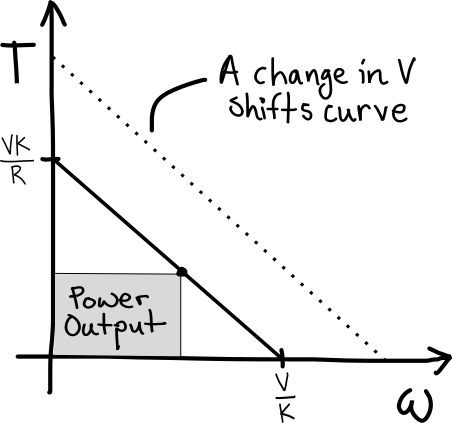
\includegraphics[width=0.4\textwidth]{Figures/MotorTorqueCurveSketch}\par
\end{centering}
\caption[Plot: Torque vs. Angular Speed for an Electric Motor]{Torque vs. angular speed for an electric motor. The relationship is linear, described by $T = \frac{k}{R}V - \frac{k^2}{R}\omega$ (equation \ref{eq:MotorTorque2}). Notice that $\frac{Vk}{R}$, the intersection of the curve and the torque axis, is directly proportional to $V$. The power developed by the motor, $T\omega$, is the area of the shaded rectangle for a given operating point.}
\label{fig:MotorTorqueCurveSketch}
\end{figure}
%

An important quantity to solve for is the free spinning angular rate $\omega_{f}$,

\begin{equation}
\omega_{f} = \frac{1}{k}V
\label{eq:FreeSpinningOmega}
\end{equation}

which is the speed at which the motor would rotate if there were no load on it. We can find the value of the motor torque constant in terms of $\omega_{f}$:

\begin{equation}
k = \frac{V}{\omega_{f}}
\label{eq:MotorTorqueConstant}
\end{equation}

where $k$ has units of \unitfrac{V}{rad/s}.

It's useful here to demonstrate the energy used by the motor:

\begin{equation}
P_{i} = VI = V\frac{T}{k} = \frac{V}{k}\left(\frac{k}{R}V - \frac{k^2}{R}\omega\right)
\label{eq:MotorPowerUse}
\end{equation}

Equation \ref{eq:MotorPowerUse} describes the power consumed by the motor, which is equal to the power supplied by the battery. This power is called the input power. This power relationship is shown in figure \ref{fig:PowerVsOmega} as a straight line, where the curved line is the output power, $P_{o}$:

\begin{equation}
P_{o} = T\omega= \left(\frac{k}{R}V - \frac{k^2}{R}\omega\right)\omega
\label{eq:MotorPowerOutput}
\end{equation}

Given the input and output power, we can calculate the motor efficiency.

\begin{equation}
\mbox{efficiency} = \frac{P_{o}}{P_{i}}
\label{eq:MotorEfficiency}
\end{equation}

At peak power, $\omega = \frac{\omega_{f}}{2}$ and the efficiency therefore equals 50\%. The peak efficiency is close to 1 when $\omega$ approaches $\omega_{f}$. The efficiency is shown in figure \ref{fig:MotorEfficiency}.

% FIGURE
\begin{figure}[h]		% h="here" t="top" b="bottom" p="separate page"
\begin{center}
 \subfloat[]{\label{fig:PowerVsOmega}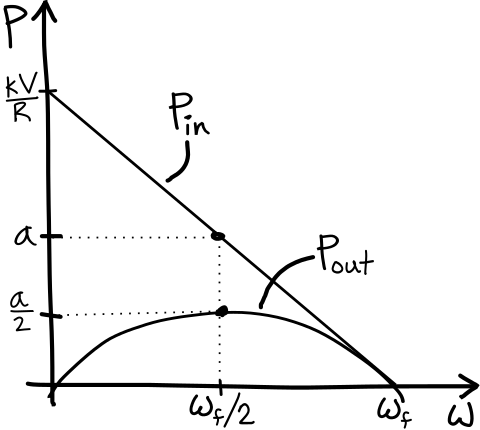
\includegraphics[width=0.38\textwidth]{Figures/PowerVsOmega}} \hspace{0.05\textwidth}%
 \subfloat[]{\label{fig:MotorEfficiency}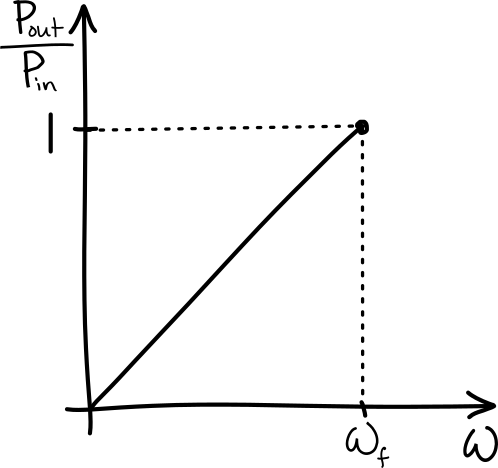
\includegraphics[width=0.33\textwidth]{Figures/MotorEfficiency}}
\end{center}
\caption[Plot: Electric Motor Power and Efficiency vs. $\omega$.] {(a) Output motor power vs. rotational speed, $\omega$. This plot shows equations \ref{eq:MotorPowerOutput} and \ref{eq:MotorPowerUse} on the same axis. The rotational speed that produces the greatest power output is half of the free spinning rotational speed of the motor. The required power drawn from the battery at this speed is twice the developed power, as indicated by the points labeled $a$ and $a/2$ on the P axis.  (b) Electric motor efficiency vs. $\omega$. An electric motor is most efficient when it is allowed to spin at its free spinning rotational speed. However, as shown in figure \ref{fig:PowerVsOmega}, the motor produces no power when it spins at its free spinning rotational speed.}
\label{fig:MotorPowerAndEfficiency}
\end{figure}
%

With our basic motor model, we can compare plots of various quantities, as in figure \ref{fig:FourMotorCurves}.

% FIGURE
\begin{figure}[h]		% h="here" t="top" b="bottom" p="separate page"
\begin{centering}
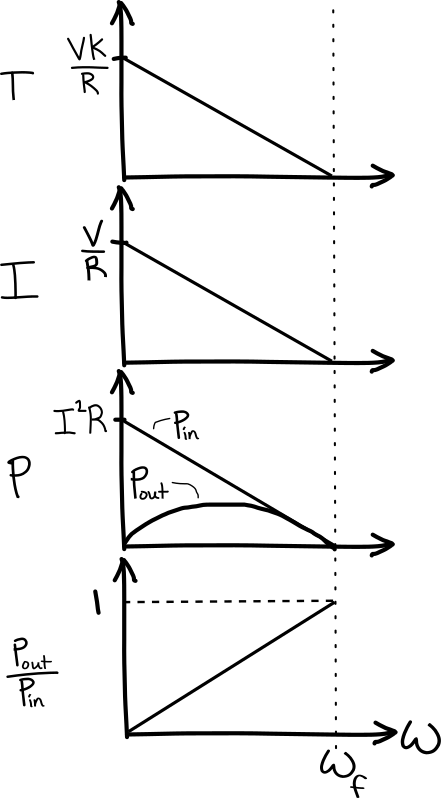
\includegraphics[width=0.35\textwidth]{Figures/FourMotorCurves}\par
\end{centering}
\caption[Plot: A Comparison of Four Motor Curves vs. $\omega$]{A comparison of motor torque, current, power, and efficiency. The torque, $T$, is a linear function of $\omega$, as is the current, $I$. The current function is simply the torque function scaled by $k$. The bottom two plots are the power and efficiency curves from figure \ref{fig:MotorPowerAndEfficiency}, shown again to emphasize that the motor produces no torque and draws no current at its free spinning rotational speed.}
\label{fig:FourMotorCurves}
\end{figure}
%

Running a motor at a low $\omega$ is not very efficient, but running a motor near free speed is very efficient. Given any motor, we can increase $V$ arbitrarily and get any power at any efficiency we choose. However, as we increase $V$ at a fixed efficiency, we also inadvertently must change $\omega$, which may not be desirable. The solution to this problem is to convert nearly free-speed rotation at the motor to a rotational speed of our choosing at our application point, e.g. at the limb of a legged robot. This scaling can be accomplished with gearboxes. A gearbox is a passive box that ideally preserves input power, or: $P_{in}=P_{out}$.

\begin{equation}
T_{in}\omega_{in} = T_{out}\omega_{out}
\label{eq:GearboxExample}
\end{equation}

% FIGURE
\begin{figure}[h]		% h="here" t="top" b="bottom" p="separate page"
\begin{centering}
 \subfloat[]{\label{fig:GearboxExample}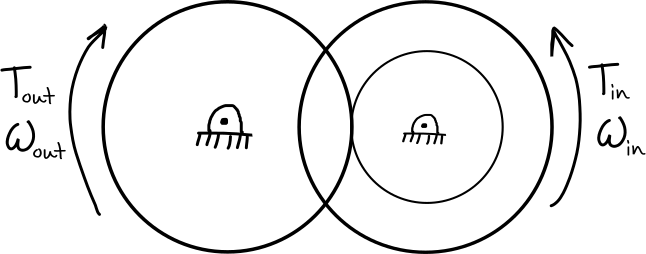
\includegraphics[width=0.5\textwidth]{Figures/GearboxExample}} \hspace{0.1\textwidth}%
 \subfloat[]{\label{fig:PulleyExample}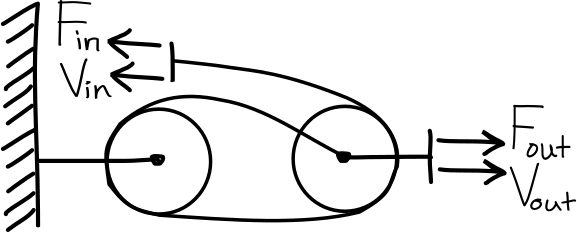
\includegraphics[width=0.4\textwidth]{Figures/PulleyExample}}
\end{centering}
\caption[Diagram: Force Amplification with Gearbox and Pulley Systems]{(a) A simple gear system. In this case, the input torque $T_{in}$ is amplified, while the input rotational speed $\omega_{in}$ is reduced ($T_{out}>T_{in}$ and $\omega_{out}<\omega_{in}$). (b) A simple pulley system. In this case, the output force is amplified, while the output velocity is reduced ($F_{out}>F_{in}$ and $V_{out}<V_{in}$). For both systems, power is conserved.}
\label{fig:GearboxAndPulleyExample}
\end{figure}
%

One drawback of gearboxes is that amplification of force (or equivalently torque) comes with a reduction in velocity. This is best illustrated with a pulley example, as in figure \ref{fig:PulleyExample}.

\begin{equation}
F_{in}v_{in} = F_{out}v_{out}
\label{eq:PulleyExample}
\end{equation}

One of the key problems in robotics is how to appropriately size a gearbox. The key equations for this problem are shown in equation \ref{eq:MotorAndGearbox}.

\begin{align}
T_{out} &=GT_{in} \notag \\
\omega_{out} &=\omega_{in}/G \notag \\
T_{in}\omega_{in}&=T_{out}\omega_{out}
\label{eq:MotorAndGearbox}
\end{align}

where $G$ is the gear ratio. These equations \ref{eq:MotorAndGearbox} neglect the presence of friction in the gearbox.

% FIGURE
\begin{figure}[h]		% h="here" t="top" b="bottom" p="separate page"
\begin{centering}
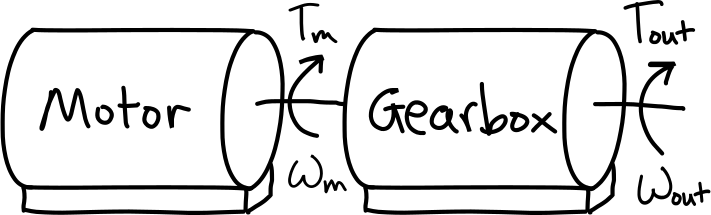
\includegraphics[width=0.5\textwidth]{Figures/MotorAndGearbox}\par
\end{centering}
\caption[Diagram: Motor Connected to a Gearbox]{A motor connected to a gearbox. The motor develops a torque $T_{m}$ and rotational speed $\omega_{m}$, which the gearbox converts into an output torque $T_{out}$ and rotational speed $\omega_{out}$. An ideal gearbox is frictionless and conserves power; the relationship between the torques and rotational speeds is described by equation \ref{eq:MotorAndGearbox}.}
\label{fig:MotorAndGearbox}
\end{figure}
%

Given any motor, $k, R$ and any efficiency, say 98\%, any power output, $P_{out}=\unit[50]{W}$, and any $\omega=\unitfrac[4]{rev}{s}$, we can pick $V$ and $G$ to do the job. However, there are some practical considerations to be aware of when choosing $V$ and $G$ for real systems.  

\begin{itemize}

\item \textbf{Motor melting.} An electric motor generates heat during operation, and can only dissipate so much heat before destroying itself.
\item \textbf{Sparking danger.} A large V could create sparking across wire leads or brush tips within the motor and cause damage to components in the motor or in the circuit that powers the motor.
\item \textbf{Real gears have friction.} The bigger the gear reduction, the more friction there is in the gearbox.
\item \textbf{Inertia.} Reflected inertia is proportional to $J_{shaft}G^{2}$.

\end{itemize}

From some of these considerations, we can build a more complete motor law.

\begin{equation}
T_{m}=kI-J\dot{\omega}_{m}
\label{eq:CompleteMotorLaw1}
\end{equation}

where the subscript $m$ denotes quantites related to the motor itself as opposed to quantities at the output of a gearbox, and $kI=T_{e}$. The voltage across the motor is

\begin{equation}
V=k\omega_{m}+IR+L\dot{I}
\label{eq:CompleteMotorLaw2}
\end{equation}

where $L$ is the inductance of the motor. The term $L\dot{I}$ allows for pulse width modulation (PWM) control of the motor. The torque provided at the output of the gearbox has the form

\begin{equation}
T_{out}=GC_{1}T_{in}-C_{2}\omega-C_{3}\frac{\omega}{|\omega|}
\label{eq:CompleteMotorLaw4}
\end{equation}

where

\begin{equation}
C_{1}=\frac{1}{1+\mu \cdot \mbox{sign}\left(T_{in}\omega_{in}\right)}
\label{eq:CompleteMotorLaw5}
\end{equation}

and $C_{2}\omega$ represents viscous friction and $C_{3}\frac{\omega}{|\omega|}$ represents dry friction. If $\mu > 1$, non-backdriveable, or if efficiency forward $< 0.5$ (50\%).

% FIGURE
\begin{figure}[htb]		% h="here" t="top" b="bottom" p="separate page"
\begin{centering}
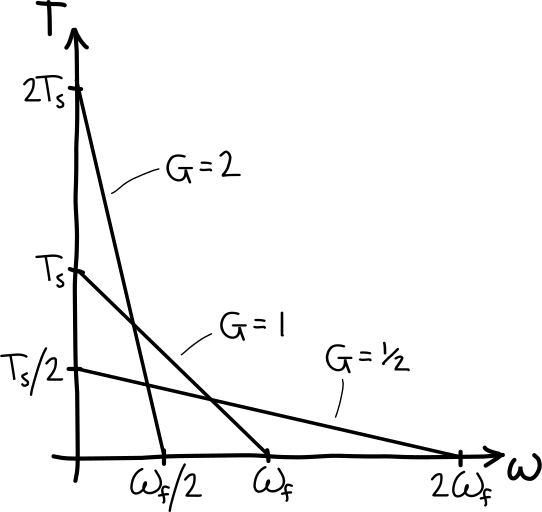
\includegraphics[width=0.4\textwidth]{Figures/GearboxCurves}\par
\end{centering}
\caption[Plot: Gearbox Torque Curves]{Gearbox torque curves. These curves are a modified version of those shown in figure \ref{fig:MotorTorqueCurveSketch}, but for different values of the gear ratio $G$. The greater the gear ratio, the greater the output torque and the smaller the output rotational speed.}
\label{fig:GearboxCurves}
\end{figure}
%

It is desireble to know the input power required to obtain a particular output power. If friction in the motor and gearbox are ignored, then the input power is a parabolic function of output power that also depends on $\omega$, k, R, and G (equation \ref{eq:GearboxPowerCurves}, figure \ref{fig:GearboxPowerCurves}). In equation \ref{eq:GearboxPowerCurves}, note that a gearbox amplifies the motor torque constant by the gear ratio. A few observations can be made from figure \ref{fig:GearboxPowerCurves}. Logically, less input power is required for a given output power as the motor resistance decreases. For low output powers, the current going through the motor is small and so the power loss from internal resistance is low and the motor is nearly 100\% efficient. 

\begin{equation}
P_{in}=P_{out}+P_{out}^{2}\frac{R}{(Gk)^{2}}
\label{eq:GearboxPowerCurves}
\end{equation}


% FIGURE
\begin{figure}[htb]		% h="here" t="top" b="bottom" p="separate page"
\begin{centering}
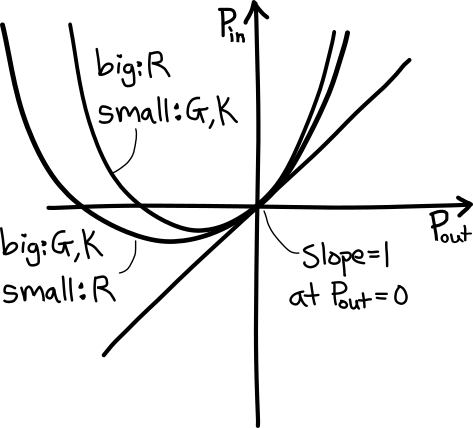
\includegraphics[width=0.4\textwidth]{Figures/GearboxPowerCurves}\par
\end{centering}
\caption[Plot: Gearbox Power Curves]{Gearbox power curves. A plot of equation \ref{eq:GearboxPowerCurves} for two different values of $R/(Gk)^2$. The curve is a parabola that intersects the origin with a slope of 1.}
\label{fig:GearboxPowerCurves}
\end{figure}
%

%%%%%%%%%%%%%%%%%%%%%%%%%%%%%%%%%%%%%%%%%%%%%%%%%

\section{Introduction to Muscles} % (notes page 7-9, 66)
\label{sec:IntroductionToMuscles}
\index{muscles}

This section is meant to serve as only a brief introduction to muscles and the mechanisms that make them work. Only a basic understanding of muscles is needed to understand the rest of the material in this book. The information presented here is a collection of bits and pieces. For a more detailed explanation of the topics discussed here, the reader should consult a basic introductory biology textbook. 

The main topic of concern for this field of study is energy use. This section introduces indirect calorimetry, metabolic efficiency, peak power consumption, the effect of slope on energy consumption, and the basic mechanisms that allow the body to move, such as muscle geometry on both a macroscopic and microscopic scale. 

\subsection{Muscle Geometry and Mechanisms}

Figure \ref{fig:HumanLeg} demonstrates some terminology that is commonly used when referring to muscles. Figure \ref{fig:HumanLeg} shows only the calf muscle of a human leg. The muscle is attached securely to the bone by tendons. Each end of the muscle is attached to different bones in the leg so that when the muscle contracts, movement is produced in the joint that connects the two bones. The calf muscle is attached to the back of the foot by the achilles tendon, and to the top of the lower leg (the tibia) just below the knee. The point where the calf attaches to the foot is called the insertion, and the point where it attaches to the tibia is called the origin. When the calf muscle contracts, a person's ankle bends and points the tip of the foot away from the rest of the leg. Since the calf muscle is located on the tibia itself, the foot is considered to be moving relative to the tibia. This relationship defines what we call the insertion and the origin; the insertion is usually the connection point on the part of the body that is moving relative to where the muscle is located. 

Animal muscles can only work in tension, so muscles must always come in pairs. To point a foot towards the knee, a muscle other than the calf muscle must contract. These pairs of muscles are called antagonistic because they pull in opposite directions of one another.  Figure \ref{fig:HumanLeg} does not show the muscle that completes the antagonistic pair with the calf muscle. 

% FIGURE
\begin{figure}[htb]		% h="here" t="top" b="bottom" p="separate page"
\begin{centering}
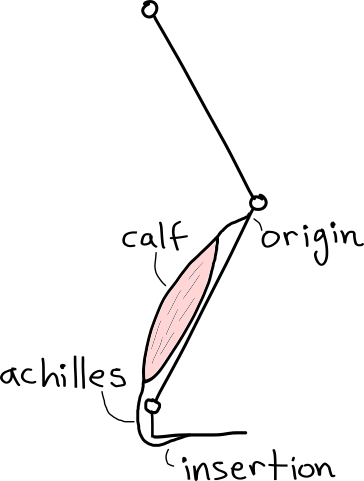
\includegraphics[width=0.3\textwidth]{Figures/HumanLeg}\par
\end{centering}
\caption[Diagram: Simple Human Leg Muscle Terminology]{Simple human leg muscle terminology. Only the calf muscle is shown, attached to bone by tendons. The origin is the point where the tendon attaches to the bone that does not move as a result of muscle contraction. The insertion is the point where the tendon attaches to the bone that is actuated by the muscle. On a human leg, the calf muscle insertion tendon is called the achilles tendon.}
\label{fig:HumanLeg}
\end{figure}
%

The tendons that connect a muscle to bone cannot actively contract. Tendons \index{tendons} are passive elastic connections from the muscle to the bone. They are only slightly elastic, but nearly perfectly so. Tendons have a small associated hysteresis \index{tendons!hysteresis} when lengthening and shortening, but this hysteresis only causes approximately 10\% of the work done during lengthening to be lost during shortening. In this regard, tendons are very similar to springs \index{tendons!springs}, and are sometimes modeled as such. Modern robots designed to replicate human locomotion sometimes incorporate stiff springs in series with an actuated cable to approximate a human muscle. 

% FIGURE
\begin{figure}[htb]		% h="here" t="top" b="bottom" p="separate page"
\begin{centering}
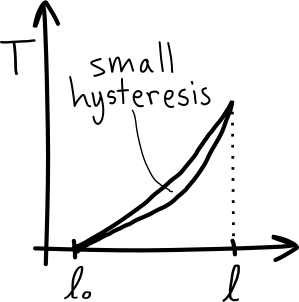
\includegraphics[width=0.25\textwidth]{Figures/TendonTensionPlot}\par
\end{centering}
\caption[Plot: Tension vs. Length for a Human Tendon]{Tension vs. Length for a human tendon. Tendons behave similarly to springs; however, there is a small hysteresis that occurs when loading and unloading tendons. The hysteresis loop forms clockwise; the tendon withstands greater force as it is being lengthened.}
\label{fig:TendonTensionPlot}
\end{figure}
%

Active contraction in muscles is the result of a microscopic structure called a sarcomere. The sarcomere is the basic functional unit responsible for muscle contraction; one muscle is made up of thousands of sarcomeres. Sarcomeres are composed of myosin and actin, intertwined as shown in figure \ref{fig:Sarcomere}. The strands, or filaments, of myosin and actin are connected by myosin heads that act as small levers. The myosin heads are part of the myson filaments, but temporarily connect to the actin filaments. When the two filaments are temporarily connected, the myosin heads bend in one direction, release, and bend back to stick to the actin again and repeat the action. This motion incrementally pulls the filaments of actin past the filaments of myosin, and the total width of the sarcomere shortens. The figure shows that there is a maximum possible contraction for any given sarcomere, and thus a maximum possible contraction for a given muscle. 

% FIGURE
\begin{figure}[htb]		% h="here" t="top" b="bottom" p="separate page"
\begin{centering}
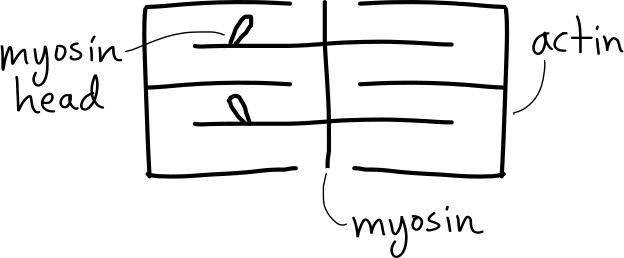
\includegraphics[width=0.35\textwidth]{Figures/Sarcomere}\par
\end{centering}
\caption[Diagram: A Sarcomere]{A sarcomere. The sarcomere is the basic functional unit responsible for muscle contraction. They are composed of myosin and actin, intertwined as shown and connected by myosin heads that act as small levers. The myosin heads connect to the actin, bend in one direction, release, and bend back to repeat the action. This motion incrementally pulls the actin closer to the myosin.}
\label{fig:Sarcomere}
\end{figure}
%

Muscles are active motors, and subsequently need fuel to operate. This fuel originally comes from caloric intake, but is spent at the muscle as a chemical called ATP (adenosine triphosphate). Only 25\% of total fuel intake goes to actual work performed by a muscle. Nearly 50\% of fuel intake is used to convert energy stored as fat to useable ATP. The process of converting fats and starches to ATP is called metabolism. Another 50\% of fuel intake is spent in the sarcomeres, converting ATP to mechanical work. Within the sarcomere, ATP and calcium ions work together to make the grab-and-release cycle happen. Calcium levels control the process, and the calcium is delivered to the muscle through a sheath that surrounds the muscle itself.

It is possible to externally stimulate muscles and force joints to actuate by applying an electric current or field to the muscle. This can be done even through the skin because an electric field can penetrate the skin and muscle tissue and cause the charged calcium ions to leave the sheath and enter the muscle. This external stimulation bypasses the normal biological process, which relies on neurons to deliver a weak electric signal to release the calcium into the muscles. 


\subsection{Muscle Energy Use}

In order to measure the energy used by muscles for locomotion we can test individual muscles for their strength or we can analyze a human as a black box that consumes energy through metabolic processes and then outputs work through locomotion. 

\subsubsection*{Indirect calorimetry}

One such black box method is called Indirect Calorimetry. This method measures the oxygen entering and carbon dioxide leaving the body, and assumes that the intermediate chemical reaction is equivalent to combustion (``burning" food). By measuring oxygen and carbon dioxide in this way, it is possible to indirectly measure the amount of food (input energy) that is used as work for locomotion. This measurement is commonly quantified by the volume of oxygen, or ``$V_{O_2}$.", inhaled. The ratio of carbon dioxide to oxygen can provide the ratio of starch to fat that is burned.

% FIGURE
\begin{figure}[htb]		% h="here" t="top" b="bottom" p="separate page"
\begin{centering}
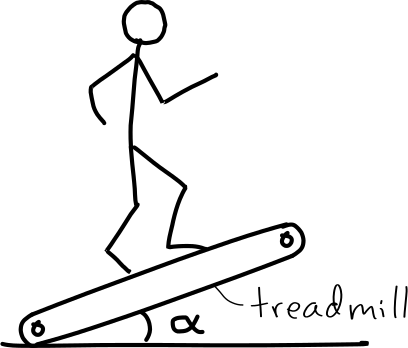
\includegraphics[width=0.35\textwidth]{Figures/Treadmill}\par
\end{centering}
\caption[Diagram: Treadmill Experiment Arrangement]{Treadmill experiment arrangement. This arrangement can be used to measure the relationship between energy use and the angle $\alpha$ of a walking surface. Increasing $\alpha$ effectively increases the amount of output work the human must perform.}
\label{fig:Treadmill}
\end{figure}
%

With a treadmill setup like the one in figure \ref{fig:Treadmill}, measurements of oxygen intake can be used to learn about the efficiency of human walking as is shown in figure \ref{fig:MetabolicCost}. As we may have garnered from experience, increasing $\alpha$ increases the amount of work the human must output to remain on the treadmill. The output work (a greater $\alpha$) requires the human to burn a certain amount of food calories (energy). This amount of energy that must be burned is the metabolic cost of locomotion. By varying $\alpha$, one can obtain different levels of output work and measure through $V_{O_2}$ the corresponding metabolic cost of that work.

% FIGURE
\begin{figure}[htb]		% h="here" t="top" b="bottom" p="separate page"
\begin{centering}
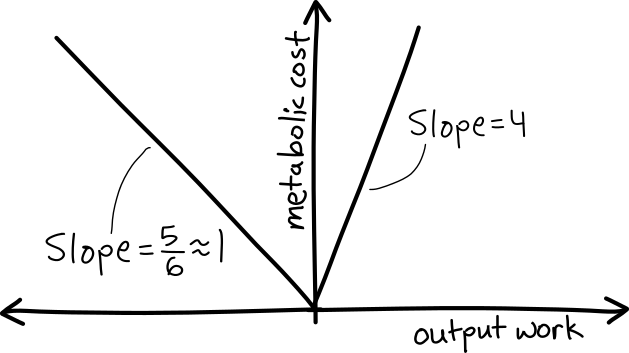
\includegraphics[width=0.5\textwidth]{Figures/MetabolicCost}\par
\end{centering}
\caption[Plot: The Metabolic Cost of Walking on a Hill]{The metabolic cost of walking on a hill.  When walking uphill, a human must input as metabolic cost approximately 4 times as much energy as the minimum energy required to move their mass uphill. Note that there is a metabolic cost for a human to walk downhill, even though a ball does not need to input energy to roll down a hill. A human must input as metabolic cost approximately 5/6 of the energy that would be created by a ball with the human's mass rolling down the hill.}
\label{fig:MetabolicCost}
\end{figure}
%

When walking uphill, the metabolic cost of locomotion associated with climbing a hill a certain distance is approximately 4 times the potential energy gained by traversing that distance. This provides an energy efficiency of $1/4 = 25\%$. For a lossless mechanism, the metabolic cost of traversing a distance up a hill would be equivalent to the output work, giving a slope of 1 in figure \ref{fig:MetabolicCost}. This is due to energy losses in converting caloric intake to fats and starches and converting those fuels into mechanical work. When walking downhill, the theoretical mechanical output work is actually negative, but humans are incapable of recovering that energy as they walk downhill. Humans still have to use metabolic energy to prevent themselves from essentially falling or tumbling downhill. The amount of energy a person spends trying to check their speed going downhill is nearly equal to the amount of energy they would gain if they were to just roll downhill. In general, the greater the incline, the more tiring it is to walk up it. The metabolic cost is linear with increases in the steepness of the slope. Also, the greater the incline, the more tiring it is to walk down it, but walking down a given incline is easier than walking up it. 

% Here's a little bit that I don't understand (AVA 20110814):

%The simplest estimate of energy cost of using muscle:
%
%\begin{align}
%P_{cost} &= C_{1}|P| \mbox{ for } P > 0\notag \\
%P_{cost} &= C_{2}|P| \mbox{ for } P < 0
%\label{eq:MetabolicCost}
%\end{align}
%
%where $C_{1}\approx0.25$ and $C_{2}\approx0.05$.

\subsubsection*{Individual muscles}

In order to determine the maximum energy or power that a muscle can exert, we need to introduce muscle strength and muscle stress.
\par
The idea that walking downhill is easier than walking uphill (for a given incline) can be observed on a smaller scale, at the muscular level. An individual muscle is also better at lowering a mass than raising a mass. Figure \ref{fig:LiftingVsLowering} shows that the amount of weight that a muscles can lower (negative work) is greater than the amount of weight that a muscle can lift (positive work). Such data is determined experimentally. The isometric strength of a muscle $T_{0}$ is how much force a muscle can provide if its length is kept fixed. Note here that the term strength is not denoting a maximum stress of a material as it does in mechanics, but a maximum force that can be exerted. The force a muscle can provide when lengthening is approximately 1.7 times the muscle's isometric strength. Also, a muscle in contraction provides less force the faster it contracts.

% FIGURE
\begin{figure}[htb]		% h="here" t="top" b="bottom" p="separate page"
\begin{centering}
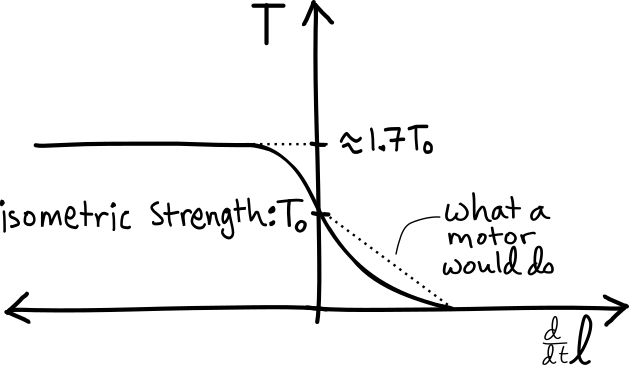
\includegraphics[width=0.5\textwidth]{Figures/LiftingVsLowering}\par
\end{centering}
\caption[Plot: Muscle Tension vs. Length Rate of Change]{Muscle tension vs. length rate of change. A muscle is capable of lowering more than it can lift. The isometric strength of a muscle $T_{0}$ describes how much force a muscle can provide with no change in length. The force a muscle can provide when lengthening is approximately 1.7 times the isometric muscle strength. A muscle in contraction provides less force the faster it contracts.}
\label{fig:LiftingVsLowering}
\end{figure}
%

Figure \ref{fig:PeakMuscleStress} is essentially the same as Figure \ref{fig:LiftingVsLowering}, except that the quantities on both axes have been normalized as is typically done in mechanics.  The isometric strength of a muscle is directly related to the peak muscle stress by a factor of the cross-sectional area of the muscle. In reality, a muscle will change cross-sectional area as it contracts, and the idea of ``stress" is only meant as a useful guide for thinking. The peak muscle stress is kind of like a muscle yield strength, except instead of yielding, the muscle simply cannot hold any more load and begins to release. For most muscles, this peak muscle stress is approximately equal to 0.1\% of the yield strength of steel.

% FIGURE
\begin{figure}[htb]		% h="here" t="top" b="bottom" p="separate page"
\begin{centering}
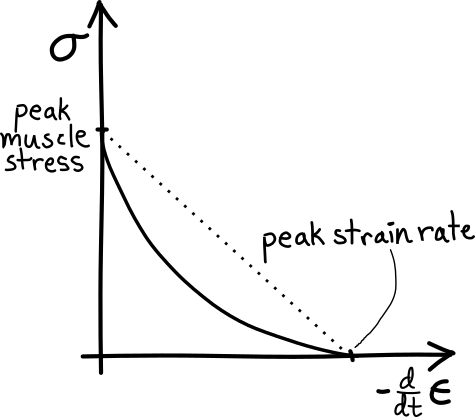
\includegraphics[width=0.4\textwidth]{Figures/PeakMuscleStress}\par
\end{centering}
\caption[Plot: Muscle Stress vs. Strain Rate]{Muscle stress vs. strain rate. The peak muscle stress can be thought of as a kind of yield strength, except instead of yielding the muscle simply cannot hold any more load and begins to release.}
\label{fig:PeakMuscleStress}
\end{figure}
%

\begin{equation}
\sigma_{peak} \approx 200 kPa
\label{eq:PeakMuscleStress1}
\end{equation}

Muscles can only operate at points on the curve in figure \ref{fig:PeakMuscleStress}, but there is bound to be an operation point at which the muscle is producing the most power it can produce. This point is at the coordinates ($\dot{\epsilon}_{peak}/3, \sigma_{peak}/3$).

\begin{equation}
\mbox{Peak Power} \approx \left(\frac{1}{3} \dot{\epsilon}_{peak}\right)\left(\frac{1}{3} \sigma_{peak}\right)
\label{eq:PeakMuscleStress2}
\end{equation}

Equation \ref{eq:PeakMuscleStress3} is a quick back-of-the-envelope calculation that shows how much power a kilogram of muscle develops. The calculation assumes a peak strain rate of $\unit[5]{s^{-1}}$, the peak muscle stress from equation \ref{eq:PeakMuscleStress1}, and a muscle density approximately that of water.

\begin{equation}
\mbox{Power/Mass} \approx \frac{\unit[5]{s^{-1}}}{3}\left(\frac{\unit[200000]{N/m^2}}{3}\right)\frac{1}{\unit[1000]{kg/m}} \approx \unit[200]{W/kg}
\label{eq:PeakMuscleStress3}
\end{equation}

In reality, the peak power is closer to \unit[50]{W/kg}. The best electric motors have a peak power/mass of approximately \unit[4000]{W/kg}, but typically they are only around \unit[200]{W/kg}. For most situations, this means that the power density of electric motors is only slightly better than that of muscle (by a factor of 4). This comparison neglects any considerations made for battery or power supply weight that might be needed to power an electric motor. 

